% arara: xelatex: { shell: yes }
% arara: biber
% arara: nomencl
% arara: xelatex: { shell: yes }
% arara: xelatex: { shell: yes }
\documentclass[ngerman]{ttlab-qualify}
% m�gliche Optionen:
% - ngerman
% - english
% - minted
% - algorithm
% - nomencl
% - nolibertine

%to export equation as png
%\usepackage[active,tightpage]{preview}
%\PreviewEnvironment{equation}

\usepackage{multirow}

\usepackage{ amssymb }
%\usepackage[captions=tableheadings]{booktabs}

\usepackage{listing} % pretty print code
\usepackage{lstbayes} % add stan languge support to listing

\usepackage{tikz}
\usepackage{subfigure}

%define Listing name Listing -> Code
\renewcommand\lstlistingname{\textit{Stan}-Code}
\renewcommand\lstlistlistingname{\textit{Stan}-Code}

\definecolor{comment}{gray}{0.50}

% lst style custom from Bertschinger, Mozzhorin, Sinha 2018
\definecolor{codeblue}{RGB}{2,88,77} %{3,135,125}
\definecolor{codegreen}{RGB}{91,117,2}%{0,0.6,0}
\definecolor{codegray}{rgb}{0.5,0.5,0.5}
\definecolor{distribution}{RGB}{201,150,3}%{0.58,0,0.82}
\definecolor{backcolour}{rgb}{0.99,0.99,0.97}

\lstdefinestyle{custom}{
  language=C++,
  literate={~}{$\sim$}{1},
  backgroundcolor=\color{backcolour},   
  commentstyle=\color{codegreen},
  otherkeywords = {real, vector, matrix, data, model, parameters, transformed},
  keywordstyle=\color{codeblue},
  numberstyle=\tiny\color{codegray},
  stringstyle=\color{distribution},
  emph={		normal, cauchy, inv_gamma, bernoulli_logit, gamma	},
  emphstyle=\color{distribution},	basicstyle={\footnotesize,\ttfamily},
  breakatwhitespace=false,         
  breaklines=true,                 
  captionpos=t,                    
  keepspaces=true,                 
  numbers=left,                    
  numbersep=5pt,                  
  showspaces=false,                
  showstringspaces=false,
  showtabs=false,                  
  tabsize=2
}

\addbibresource{bib/bayes.bib}
\usepackage{float} %use [H]with figure to place figures right in the text
 
\usepackage[colorlinks=false,
pdfpagelabels,
pdfstartview = FitH,
bookmarksopen = true,
bookmarksnumbered = true,
%urlcolor = blue,   %externe URLs
%linkcolor = black, %interne Verweise
%citecolor = blue,  %interne Zitate
urlbordercolor={0.5 0.5 0.5},
linkbordercolor={0.5 0.5 0.5},
citebordercolor={0.5 0.5 0.5},
plainpages = false,
hypertexnames = true]{hyperref}
%insert links from title back to toc
\makeatletter
\let\hyperchapter\chapter
\def\chapter{\@ifstar\starchapter\mychapter}
\def\starchapter{\hyperchapter*}
\newcommand{\mychapter}[2][\@empty]% #1=optional (toc and top of page), #2=title
{\ifx#1\@empty \hyperchapter[#2]{\hyperlink{toc.chapter.\thechapter}{#2}}
 \else \hyperchapter[#1]{\hyperlink{toc.chapter.\thechapter}{#2}}
 \fi}

\let\hypersection\section
\def\section{\@ifstar\starsection\mysection}
\def\starsection{\hypersection*}
\newcommand{\mysection}[2][\@empty]% #1=optional (toc), #2=title
{\ifx#1\@empty \hypersection[#2]{\hyperlink{toc.section.\thesection}{#2}}
 \else \hypersecton[#1]{\hyperlink{toc.section.\thesection}{#2}}
 \fi}
 
 \let\hypersubsection\subsection
\def\subsection{\@ifstar\starsubsection\mysubsection}
\def\starsubsection{\hypersubsection*}
\newcommand{\mysubsection}[2][\@empty]% #1=optional (toc), #2=title
{\ifx#1\@empty \hypersubsection[#2]{\hyperlink{toc.subsection.\thesubsection}{#2}}
 \else \hypersubsecton[#1]{\hyperlink{toc.subsection.\thesubsection}{#2}}
 \fi}
\makeatother
%change u.a. to et.al. - edit E. Fughe 4.7.18
\DefineBibliographyStrings{ngerman}{
   andothers = {{et\,al\adddot}},
}

\begin{document}
\let\hypercontentsline=\contentsline
\renewcommand{\contentsline}[4]{\hypertarget{toc.#4}{}\hypercontentsline{#1}{#2}{#3}{#4}}

\titlehead{
  Elisabeth Fughe\\
  Matrikelnummer: 5263769\\
  s3499227@stud.uni-frankfurt.de
}
\subject{Bachelorarbeit (B.Sc. - Informatik)}
\author{Elisabeth Fughe}
\title{Können Modelle der Ökonophysik Preis-Dynamiken vorhersagen?}
\subtitle{Fitting von Markt-Modellen auf empirischen Daten mittels Bayesscher Statistik}
\date{Abgabedatum: 16. April 2019}
\publishers{FIAS - Frankfurt Institute for Advanced Studies\\Prof. Dr. Nils Bertschinger}
%\\Ggf. Name des Zweitbetreuers}

\maketitle

\chapter*{Zusammenfassung}
tbd

\tableofcontents
\listoffigures
%\listoftables

\chapter{Einleitung}
\label{chap:summary}
tbd

\chapter{Verwendete Methoden}
\label{chap:methoden}
In den nachfolgenden Kapiteln~\ref{chap:bayes} bis~\ref{chap:stan} werden die mathematischen Grundlagen, die verwendeten Methoden sowie die Programmiersprache erläutert. Um verschiedene Modelle auf den gleichen Daten anzuwenden und vergleichen zu können, wurden die Modelle von Bertschinger, Mozzhorin und Sinha \parencite{bertschinger:2018} in der Programmiersprache \textit{Stan} beschrieben. Anschließend ist das Fitten der Modelle auf den Daten mittels \textbf{R} leicht umsetzbar.
\section{Bayessche Modellierung}
\label{chap:bayes}
Die Bayessche Statistik untersucht mittels Bayesscher Wahrscheinlichkeiten und dem Satz von Bayes Fragestellungen der Stochastik. Anders als in der klassischen Statistik, die unendlich oft wiederholbare Zufallsexperimente voraussetzt, steht die Verwendung und Modellierung von Wahrscheinlichkeitsverteilungen im Vordergrund. \\
Es gilt, dass beobachtete Daten 
\[x=(x_1,...,x_n)\] 
mittels bedingter Wahrscheinlichkeiten in Beziehung zu unbekannten Parametern 
\[\theta = (\theta_1,...,\theta_m)\] 
stehen. So kann die gemeinsame Wahrscheinlichkeitsdichte 
\[p(x,\theta) = p(x\theta)\cdot p(\theta)\]
durch die a-priori-Verteilung unbekannter Parameter $p(\theta)$ und den Erkenntnissen aus dem Datensatz $p(x|\theta)$ berechnet werden.
Mit Hilfe des Satzes von Bayes kann dann die a-posteriori-Verteilung unbekannter Parameter 
\[p(\theta|x) =\dfrac{p(x|\theta)\cdot p(\theta)}{p(x)}\] 
ermittelt werden \parencite{bertschinger:2018}.

Die a-posteriori-Verteilung enthält somit Informationen über die unbekannten Parameter durch die Kombination der a-priori Verteilung mit den Informationen, die aus den beobachteten Daten gewonnen wurden. Sie wird zur Punktschätzung und zur Schätzung von Konfidenzintervallen genutzt und daher auch oft als Ziel-Verteilung bezeichnet.

So sind Bayessche Modelle im Gegensatz zur klassischen Statistik auf kleineren Datensätzen anwendbar, dort ergibt sich jedoch eine breite Wahrscheinlichkeitsverteilung, die somit unter Umständen eine geringe Genauigkeit aufweist.

\section{Markov Chain Monte Carlo (MCMC)}
\label{chap:MCMC}
In der Bayesschen Statistik beschreibt die a-posteriori-Verteilung die Unsicherheit der unbekannten Parameter, die anhand beobachteter Daten geschätzt wurden. Mit der Markov Chain Monte Carlo (MCMC) Methode können die a-posteriori-Verteilung und dadurch die unbekannten Parameter untersucht werden \parencite{hanson:2001}.

Um aus der Ziel-Verteilung Stichproben ziehen zu können, wird eine Markov-Kette entworfen, deren stationäre Verteilung der Ziel-Verteilung entspricht. Hier wird eine Stichprobe aus der a-posteriori-Wahrscheinlichkeitsdichte benötigt, sodass das langfristige Gleichgewicht der Markov-Kette der a-posteriori-Wahrscheinlichkeitsdichte entspricht. Der Zustand der Markov-Kette, der sich möglichst nah am Gleichgewicht befindet, entspricht dann einem Element der Stichprobe. Es gilt somit, dass sich die Qualität der Stichprobe mit der Anzahl der Schritte, die die Markov-Kette zurücklegt, verbessert.\\

Zur Konstruktion der Markov-Kette wird eine Übergangsfunktion berechnet, die die Ziel-Wahrscheinlichkeitsdichte invariant lässt, damit die Ziel-Dichte der stationären Verteilung der Markov-Kette entspricht. 
Sei z.B. $p(\theta)$ die Ziel-Dichte und sei $t(\theta^{'}|\theta)$ die Übergangsdichte, dann gilt
\[p(\theta^{'}) =\int t(\theta^{'}|\theta)\cdot p(\theta) d\theta \]

Stellt man sich die Markov-Kette als zufällig durch einen Parameterraum, also z.B. die a-posteriori-Verteilung, wandernden Punkt vor, so entspricht die $n$-te Komponente der Verteilung der relative Wahrscheinlichkeit, den Punkt im Zustand $n$ anzutreffen. 
%insert figure from betancourt:2017
\begin{figure}[h]
\begin{center}
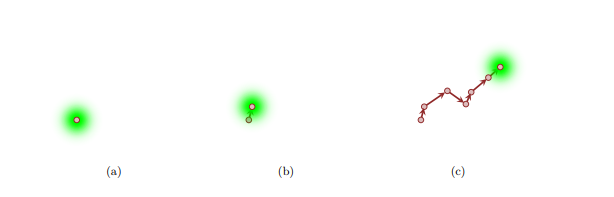
\includegraphics[scale=.9]{images/markov-chain-plain-betancourt-2017}
\caption{Verhalten der Markov-Kette beim Ziehen von Stichproben \parencite{betancourt:2017}}
\label{fig:markov-chain-plain}
\end{center}
\end{figure}

Die Übergangsdichte (grün) (a) in Abbildung~\ref{fig:markov-chain-plain} beschreibt die Wahrscheinlichkeit eines neuen Punktes im Parameterraum in Abhängigkeit der aktuellen Position d.h. die Wahrscheinlichkeit des nächsten Schrittes der Markov-Kette auf ihrem Weg durch die Verteilung in Abhängigkeit ihrer aktuellen Position.  Werden Stichproben aus dieser Verteilung gezogen, also wurden zufällig gewählte nächste Schritte vom Algorithmus akzeptiert, ergibt sich ein weiterer Zustand in der Markov-Kette und eine neue Verteilung, von der Stichproben gezogen werden können (vgl. (b) in Abbildung~\ref{fig:markov-chain-plain}). So wandert die Markov-Kette durch den Parameterraum (c) (vgl. Abbildung~\ref{fig:markov-chain-plain}).

\begin{figure}[H]
\begin{center}

\includegraphics[scale=.9]{images/markov-chain-target-betancourt-2017}
\caption{Konzentration der Markov-Kette auf die typische Menge einer Verteilung \parencite{betancourt:2017}}
\label{fig:markov-chain-target}
\end{center}
\end{figure}

Wenn die Übergangsdichte die Ziel-Verteilung beibehalten soll, konzentriert sie sich auf deren typische Menge\footnote{\textbf{Typical Set (hier: typische Menge):} Die typische Menge ist ein Begriff aus der Informationstheorie und hängt direkt mit dem Begriff der Entropie zusammen. Es gilt, dass die Summe aller Wahrscheinlichkeiten aller Elemente der typischen Menge annähernd 1 ist \parencite{typical_set}. Daher enthält die typische Menge eine gute Beschreibung des Parameterraums.} (rot) siehe Abbildung~\ref{fig:markov-chain-target}. 
Unter idealen Bedingungen entdeckt die Markov-Kette in drei verschiedenen Phasen:
\begin{enumerate}
\item Die Markov-Kette konvergiert gegen die typische Menge der Verteilung. Die MCMC-Schätzer sind stark verzerrt.
\item Die Markov-Kette hat die typische Menge erkannt und verweilt dort. Diese erste Erkundung der typischen Menge ist äußerst effektiv und verringert die Verzerrung der MCMC-Schätzer erheblich, da die Verzerrung der ersten Stichproben eliminiert wird.
\item In der dritten Phase wird die Präzision der MCMC-Schätzer durch weiteres Erforschen der typischen Menge weiter verfeinert, so dass sie den zentralen Grenzwertsatz erfüllen. Das bedeutet, dass die durch die Markov-Kette gezogenen Stichproben asymptotisch der Ziel-Verteilung folgen.
\end{enumerate}

Ideale Bedingungen liegen allerdings nicht vor, wenn die typische Menge der a-posteriori-Verteilung z.B. eine starke Krümmung aufweist (siehe Abbildung~\ref{fig:markov-chain-curve}). Die Markov-Kette kann damit nicht umgehen und aus diesem stark gekrümmten Bereich keine Stichprobe ziehen und ignoriert diesen einfach und verzerrt dadurch die MCMC-Schätzer. 
Da Markov-Ketten die exakten Erwartungen asymptotisch wiederherstellen müssen, ist eine Kompensation dafür nötig, dass manche Regionen der Ziel-Verteilung nicht beachtet wurden. Dazu bleibt die Markov-Kette an der Grenze der Krümmung hängen. So werden die MCMC-Schätzer annähernd so berechnet, als würde die Markov-Kette den gekrümmten Bereich erkunden. Allerdings erhält man so überschätzte MCMC-Schätzer.
Eine starke Krümmung in der typischen Menge der Ziel-Verteilung führt also zu verzerrten MCMC-Schätzern, die den zentralen Grenzwertsatz nicht mehr erfüllen \parencite{betancourt:2017}.

\begin{figure}[H]
\begin{center}

\includegraphics[scale=.9]{images/markov-chain-curve-betancourt-2017}
\caption{Starke Krümmungen (grün) der typischen Menge einer Verteilung führen zu verzerrten MCMC-Schätzern \parencite{betancourt:2017}}
\label{fig:markov-chain-curve}
\end{center}
\end{figure}


%----

%Anschließend wird diese Markov-Kette solang simuliert bis sie, mit einer entsprechenden Sicherheit, das Gleichgewicht erreicht hat. Dann wird der finale Zustand der Markov-Kette als Teil der Stichprobe notiert \parencite{kendall:2005}. Die Markov-Kette generiert so eine Reihe von Modell-Realisierungen, die zufällig aus der a-posteriori-Verteilung gezogen werden \parencite{hanson:2001}.\\

Ein weit verbreitetes MCMC-Verfahren zur Konzentration auf die typische Menge der zu untersuchenden Verteilung ist der Metropolis-Hastings-Algorithmus. Der Algorithmus startet an einem zufälligen Punkt in der zu untersuchenden Verteilung.
Dann wird eine Schrittweite zufällig mit Hilfe einer symmetrischen Wahrscheinlichkeitsverteilung gewählt.
Der Schritt wird auf Grundlage der Wahrscheinlichkeit der neuen Position im Verhältnis zur alten Position abgelehnt oder akzeptiert \parencite{hanson:2001}.
So wird sicher gestellt, dass die Markov-Kette von jedem Punkt aus gegen das langfristige Gleichgewicht der Ziel-Wahrscheinlichkeitsdichte konvergiert \parencite{bertschinger:2018}.\\

Der Metropolis-Hastings-Algorithmus ist sehr einfach zu implementieren und liefert gute Ergebnisse, allerdings nicht bei stark korrelierten Parametern \parencite{hanson:2001} und hoher Komplexität der Verteilung \parencite{betancourt:2017}.  Denn wenn die a-posteriori-Verteilung stark gekrümmt ist, bleibt die Markov-Kette an diesen Rändern hängen und lehnt so gut wie jeden weiteren Schritt ab. So kann nicht aus allen Bereiche der Ziel-Verteilung Stichproben gezogen werden und es entsteht eine verzerrte Stichprobe.\\
Je mehr Dimensionen die Verteilung hat, desto kleiner wird die typische Menge der Verteilung. Das führt dazu, dass fast immer Punkte außerhalb der typischen Menge gewählt werden. Die Dichte des Punktes ist so klein, dass der Schritt vom Metropolis-Hastings-Algorithmus immer abgelehnt wird. Das führt dazu, dass sich die Markov-Kette kaum weiter bewegt. Erhöht man die Akzeptanz, indem man die Anzahl der Punkte reduziert, die sich in der typischen Menge befinden müssen, führt das dazu, dass die Markov-Kette extrem langsam konvergiert \parencite{betancourt:2017}. In der Theorie würde die Markov-Kette das langfristige Gleichgewicht erreichen, aber in der Praxis stehen dazu nicht unendliche Ressourcen zur Berechnung zur Verfügung. \\
%not sure
Der Metropolis-Hastings-Algorithmus kann auch als stochastisches Optimierungsverfahren verstanden werden. Mittels Simulated Annealing\footnote{\textbf{Simulated Annealing:} \glqq Ein heuristisches Approximationsverfahren. Es wird zum Auffinden einer Näherungslösung von Optimierungsproblemen eingesetzt, die durch ihre hohe Komplexität das vollständige Ausprobieren aller Möglichkeiten und mathematische Optimierungsverfahren ausschließen\grqq \parencite{simulated_annealing}.} nähert man sich mit immer höherer Wahrscheinlichkeit an ein Minimum an. Ist die Krümmung der Verteilung zu stark, kann der Algorithmus das lokale Minimum nicht mehr verlassen und so wird fast jeder weitere Schritt der Markov-Kette abgelehnt. Letztlich wird der Bereich der Verteilung ignoriert bzw. die Markov-Kette bleibt am Rand des unerwarteten Bereichs hängen. Das führt zu einer Verzerrung der resultierenden MCMC-Schätzer \parencite{betancourt:2017}.

\section{Hamiltonian Monte Carlo Sampling (HMC)}
\label{chap:HMC}
In Modellen mit vielen Dimensionen ist es möglich, dass die Markov-Kette mittels Metropolis-Hastings-Algorithmus nicht alle Bereiche der Ziel-Verteilung in einer angemessenen Zeit abtasten kann. 
Die Strategie des Metropolis-Algorithmus, zufällige Schritte zu wählen und danach zu entscheiden, ob der Schritt akzeptiert wird oder nicht, ist für Modelle mit vielen Dimensionen weniger erfolgreich. Denn es existieren exponentiell viele Richtungen, in die sich der Sampler bewegen kann, aber nur ein Bruchteil der Richtungen belässt den Sampler in der typischen Menge und führt letztlich zu akzeptieren Stichproben.\\

Um große Schritte vom initialen Punkt in unentdeckte Bereiche der Ziel-Verteilung machen zu können, müssen Informationen über die Geometrie der Verteilung genutzt werden. Die Markov-Kette soll Übergänge berechnen, die der Masse mit hohen Wahrscheinlichkeiten folgt, sich also zusammenhängend durch die typische Menge bewegen. Diese Hamiltonian-Markov-Übergänge können durch Nutzung der differenzierbaren Struktur der a-posteriori-Verteilung berechnet werden.\\

\begin{figure}[H]
\begin{center}
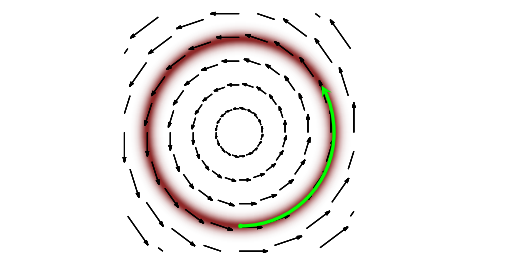
\includegraphics[scale=.9]{images/vector-field-plain-betancourt-2017}
\caption{Mit Hilfe eines Vektorfeldes das an der typischen Menge ausgerichtet ist, kann die Ziel-Verteilung leichter abgetastet werden \parencite{betancourt:2017}.}
\label{fig:vec-field-plain}
\end{center}
\end{figure}

Um die Zielverteilung schneller und gezielter abtasten zu können, wird jedem Punkt im Parameterraum eine Richtung für eine kleine Distanz zugewiesen, z.B. durch ein Vektorfeld, dass an der typischen Menge ausgerichtet ist (vgl. Abbildung~\ref{fig:vec-field-plain}). Folgt der Sampler den Richtungen, entsteht eine zusammenhängende Kurve (\textit{engl. Trajectory}), die effizient und möglichst schnell vom initialen Punkt durch unentdeckte Bereiche  der typischer Menge der Ziel-Verteilung führt \parencite{betancourt:2017}.\\

Um jedem Punkt eine Richtung zuzuweisen, kann ein Vektorraum mittels Informationen der Ziel-Verteilung konstruiert werden. Dazu wird die differenzielle geometrische Struktur der a-posteriori-Verteilung benötigt, die wir durch den Gradienten der Ziel-Dichte erhalten können. Denn der Gradient der Ziel-Dichte definiert eben ein solches für die geometrische Struktur der Verteilung sensitives Vektorfeld im Parameterraum.

\begin{figure}[H]
\begin{center}
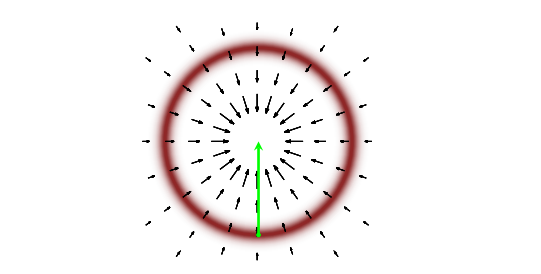
\includegraphics[scale=.9]{images/vector-field-grad-betancourt-2017}
\caption{Die Richtung des Gradienten zeigt immer von der typischen Menge in Richtung parameter-sensitiver Bereiche(grüner Pfeil), wie z.B. dem Modus der Verteilung. Folgt der Sampler diesen Richtungen, kann er die typische Menge nicht erkunden \parencite{betancourt:2017}.}
\label{fig:vec-field-grad}
\end{center}
\end{figure}

Allerdings hängen Ziel-Dichte sowie ihr Gradient stark von den Verteilungsparametern ab, sodass der Gradient immer in Richtung parameter-sensitiver Bereiche wie z.B. dem Modus\footnote{\textbf{Modus:} Der Modus ist ein Begriff der desktiptiven Statistik. Er entspricht dem häufigsten Wert einer Stichprobe \parencite{modus}.} der Verteilung zeigt (vgl. Abbildung~\ref{fig:vec-field-grad}).
Das Vektorfeld enthält somit nicht genügend Informationen, um den Sampler durch die typische Menge in parameter-invariante Bereiche zu führen. Um parameter-invariante Bereiche der Ziel-Dichte zu erkunden, muss der Gradient um zusätzliche geometrische Informationen ergänzt werden. \\

Das Ergänzen der Informationen ist durch Differentialgeometrie möglich, die auch die Mathematik der klassischen Physik beschreibt. Es gilt, dass für jedes probabilistische System ein mathematisch äquivalentes physikalisches System existiert \parencite{betancourt:2017}.
Das Erkunden der Ziel-Dichte kann äquivalent auch als Erkunden eines physikalischen Systems beschrieben werden. Sei der Modus der Ziel-Dichte ein Planet und der Gradient sein Gravitationsfeld, dann sei die typische Menge der Dichte, der Bereich um den Planeten, durch den ein Satellit kreisen soll (vgl. Abbildung~\ref{fig:vec-field-sat}). \\

\begin{figure}[H]
\begin{center}

\includegraphics[scale=.9]{images/vector-field-sat-betancourt-2017}
\caption{Analoges System der klassischen Physik \parencite{betancourt:2017}.}
\label{fig:vec-field-sat}
\end{center}
\end{figure}

Es gilt also das probabilistische Modell so um Impulse (\textit{engl. Momentum}) zu erweitern, dass analog der Satellit die Anziehungskraft des Planeten ausbalanciert und die gewünschte Umlaufbahn nicht verlässt \parencite{betancourt:2017}. Der Hamiltonian Monte Carlo Algorithmus ist der einzige Algorithmus, der Impulse mit einer probabilistischen Struktur, die konservative Dynamiken erlaubt, implementiert \parencite{betancourt:2017}.\\

Der HMC-Algorithmus zieht also Stichproben aus einem erweiterten Zustandsraum mit Impuls $i$ eines Teilchens an der Position $P$.\\
Für die Dichte $d(P,i)$ des Zustandsraums gilt \parencite{bertschinger:2018}:
\begin{align}
d(P,i)&= d(P)d(i|P)\nonumber\\
&=e^{log\; d(P)+log\; d(i|P)}\nonumber\\
&=e^{-H(P,i)}
\end{align}
Wobei die Hamiltonian-Korrektur $H(P,i)$ in Analogie zum physikalischen System der Summe potentieller und kinetischer Energie entspricht.
\[H(P,i) = -log\; d(P)-log\; d(i|P)\]
Die Hamiltonian Dynamiken $\hat{P}$ und $\hat{i}$
\begin{align} \label{eq:hamiltonian-dynamics}
\hat{P}&= \frac{\partial}{\partial i}H(P,i) \nonumber\\
&= -\frac{\partial}{\partial i} log\; d(i|P) \nonumber \\
&\nonumber\\
\hat{i}&=-\frac{\partial}{\partial P}H(P,i)\nonumber\\
&=\frac{\partial}{\partial P}log\; d(P) + \frac{\partial}{\partial P}log\; d(i|P)
\end{align}
erhalten die gesamte Energie bzw. Wahrscheinlichkeit und so kann beim HMC Sampling stets ein Schritt berechnet werden, der akzeptiert wird \parencite{bertschinger:2018}, sodass die Markov-Kette auch aus stark gekrümmten Bereichen akzeptierte Stichproben ziehen kann. Besonders in Modellen mit vielen Dimensionen schafft das HMC Sampling so wichtige Effizienzvorteile.\\

Theoretisch ist HMC Sampling unempfindlich bezüglich stark korrelierter Parameter, allerdings werden die Differenzialgleichungen in der Praxis mittels endlicher Schrittweite gelöst. Das kann dazu führen, dass stark gekrümmte Bereiche der Ziel-Dichte doch nicht mehr erreicht werden. Außerdem gilt es die Schrittweite entsprechend der Parameter-Maßeinheiten und -Größen anzupassen \parencite{bertschinger:2018}. 

\section{\textit{Stan} und \textit{R}}
\label{chap:stan}
\textit{Stan} ist eine Open-Source Plattform für statistische Modellierung und high-performance Berechnungen. 
\textit{Stan} ist für alle in der Datenanalyse weit verbreiteten Sprachen (R, Python, shell MATLAB, Julia, Stata) verfügbar und läuft auf den gängigen Betriebssystem (Linux, Mac, Windows) \parencite{stan:2017}. \\

\textit{Stan} ist eine höhere Programmiersprache und ermöglicht die Beschreibung der gemeinsamen Verteilung eines Modells auf einer hohen Abstraktionsebene. Die Sprache unterstützt viele Inferenz-Algorithmen, insbesondere Algorithmen, die das Gradientenabstiegsverfahren nutzen, um eine maximale a-posteriori-Schätzung zu erhalten, HMC Sampling sowie Bayessche Gradientenvariation (stochastic gradient variational Bayes). \textit{Stan} Code wird in C++ kompiliert und die hohe Abstraktionsebene der Sprache bietet dem Nutzer einige Vorteile, z.B. müssen bei der Nutzung von HMC Sampling die Gradienten nicht manuell implementiert werden. Benötigte Gradienten werden built-in mittels C++ Library für automatisches Differenzieren berechnet \parencite{bertschinger:2018}.\\

Ein \textit{Stan}-Programm muss mindestens einen \verb|data|-, einen \verb|Parameter|-Block sowie einen \verb|model|-Block enthalten.
Ein Beispiel dafür ist der \textit{Stan}-Code des in dieser Arbeit verwendeten GARCH-Modells:\\

Im \verb|data|-Block wird definiert, welche Daten benötigt werden, um das Modell zu fitten. Die Variablen in diesem Block entsprechen also den tatsächlichen Beobachtungen und der Block definiert, in welchem Format diese Daten vorliegen.\\
Hier wird zum Beispiel ein Vektor mit Zeitpunkten \verb|T|, ein Vektor mit Angabe, ob es sich um eine tatsächliche Beobachtung oder um einen zu vorhersagenden Wert handelt, oder einen Vektor der beobachtete Returns in jedem Zeitpunkt enthält, erwartet.\\

Im \verb|transformed data| Block können berechnete Daten/Variablen definiert werden. Hier zum Beispiel wird über die Daten iteriert und festgestellt, wie viele Einträge als \textit{Missing Value} markiert wurden. So werden Beobachtungen und Vorhersagen bzw. die zu vorhersagende Daten unterschieden.

\begin{lstlisting}[style=custom]
data {
  int<lower=0> T;
  int<lower=0, upper=1> miss_mask[T];
  real ret_obs[T]; // Note: Masked indices treated as missing
}
transformed data {
  int N = 0; // number of missing values
  for (t in 1:T)
    if (miss_mask[t] == 1) N = N + 1;
}

\end{lstlisting}

Daran anschließend kommt der \verb|parameters|-Block, der die unbekannten Parameter des Modells definiert. Anschließend daran kann der \verb|transformed parameters|-Block dazu genutzt werden, um z.B. die Berechnungsvorschrift weiterer Parameter festzulegen.\\

Hier wird der Return für jeden Zeitpunkt \verb|T| berechnet: Handelt es sich um eine tatsächliche Beobachtung, wird der beobachtete Return genommen, ansonsten erfolgt die Berechnung mit Hilfe der Standardabweichung im aktuellen Zeitpunkt berechnet:\\
\verb|ret[t] = mu + sigma[t] * eps_miss[t]|

\begin{lstlisting}[style=custom]
parameters {
  real mu;
  real<lower=0> alpha0;
  real<lower=0,upper=1> alpha1;
  real<lower=0,upper=(1-alpha1)> beta1;
  real<lower=0> sigma1;
  real eps_miss[N]; // missing normalized return innovations
}
transformed parameters {
  real ret[T]; // returns: observed or r_t=mu+sigma_t*eps_t
  real<lower=0> sigma[T];

  {
    int idx = 1; // missing value index

    sigma[1] = sigma1;
    if (miss_mask[1] == 1) {
      ret[1] = mu + sigma[1] * eps_miss[idx];
      idx = idx + 1;
    } else
      ret[1] = ret_obs[1];

    for (t in 2:T) {
      sigma[t] = sqrt(alpha0
                    + alpha1 * pow(ret[t - 1] - mu, 2)
                    + beta1 * pow(sigma[t - 1], 2));
      if (miss_mask[t] == 1) {
        ret[t] = mu + sigma[t] * eps_miss[idx];
        idx = idx + 1;
      } else
        ret[t] = ret_obs[t];
    }
  }
}
\end{lstlisting}

Zum Schluss kommt der \verb|model|-Block, der die Berechnungsvorschrift der Wahrscheinlichkeitsdichte des Modells enthält \parencite{stan:2017}.\\
Hier die Annahme, dass \verb|mu| und \verb|sigma| standardnormalverteilt sind. Die Returns sind normalverteilt zu den Parametern des Modells (\verb|mu|, \verb|sigma|) wobei es sich, um die Standarabweichung in jedem Zeitpunkt \verb|T| handelt. Weitere Erläuterungen befinden sich im Kapitel~\ref{chap:garch} \\

Anschließend daran können im \verb|generated quantities|-Block weitere Berechnungen definiert werden. 
Hier z.B. die Berechnungsvorschrift der bedingten gemeinsamen Wahrscheinlichkeitsdichte.

\begin{lstlisting}[style=custom]
model {
  mu ~ normal(0, 1);
  sigma1 ~ normal(0, 1);

  ret ~ normal(mu, sigma);
  // Jacobian correction for transformed innovations
  for (t in 1:T) {
    if (miss_mask[t] == 1)
      target += log(sigma[t]);
  }
}
generated quantities {
  real log_lik[T];

  for (t in 1:T)
    log_lik[t] = normal_lpdf(ret_obs[t] | mu, sigma[t]);
}

\end{lstlisting}

Der \textit{Stan}-Code der Modelle, die in dieser Arbeit genutzt wurden befindet sich im Anhang und wird im Kapitel~\ref{chap:models} näher erläutert.

Die Modelle wurden mittels \textit{Rstan} in \textit{R} gefittet. \textit{Rstan} ermöglicht es \textit{Stan}-Modelle in \textit{R} zu kompilieren, zu testen und zu analysieren. 
Außerdem wurden die Pakete \textit{tidybayes} und \textit{tidyverse} genutzt, um die Plots zu generieren. Die tidy* Pakete zeichnen sich dadurch aus, dass sie der komplexen Datenstruktur des berechneten Fits, Informationen leicht entnehmen können und in einer Datenstruktur zur Verfügung stellen, die anschließend z.B. mittels \textit{ggplot}-Packet leicht in \textit{R} visualisiert werden kann.

\chapter{Die Modelle}
\label{chap:models}
In den letzten Jahren haben agentenbasierte Asset-Pricing-Modelle an Bedeutung gewonnen. Im Gegensatz zur Rationalitätsannahme des Homo oeconomicus, werden nur einfache heuristische Strategien über das Verhalten von Marktteilnehmern getroffen.

Gemeinsamkeiten: readme.txt -> log returns, input, parameter, ....\\
stan data und parameter block beschreiben - dann pro kapitel nur die abweichenden Code lines zeigen\\
jacobian correction erklären\\
agent-based + GARCH als Vergleich

\section{Generalized Autoregressive Conditional Heteroscedasticity (GARCH)}
\label{chap:garch}
Generalisierte autoregressive bedingte Heteroskedastizitäts-Modelle sind stochastische Modelle zur Zeitreihenanalyse. 

Autoregressive Modelle beschreiben Beobachtungen als Kombination linearer Abhängigkeit von sich selbst sowie einer Zufallsvariable z. B. zufällige Modellfehler. Die Zufallsvariable ist entsprechend nur unter Unsicherheit vorhersagbar. Mit Hilfe von autoregressiven Modellen wird also untersucht inwiefern Beobachtungen in einem Zeitpunkt von der Vergangenheit abhängen.

Autoregressive bedingte Heteroskedastizitäts-Modelle kurz ARCH-Modelle wurden erstmals von Robert F. Engle im Jahr 1982 beschrieben. ARCH($i$)-Modelle treffen die Annahme, dass die bedingte Varianz der zufälligen Modellfehler im Zeitpunkt $t$ vom realisierten Zufallsfehler der letzten $i$ Vorperioden abhängt. Das heißt, dass große bzw. kleine Fehler dazu neigen in Clustern aufzutreten \parencite{engle:1982}.

Heteroskedastizität ist ein Begriff der Statistik, der die Streuung innerhalb eines Datensatzes beschreibt. Heteroskedastizität liegt in einer Zeitreihe dann vor, wenn die Abweichung der Daten von einer Trendgeraden im Zeitverlauf zu bzw. abnimmt oder auch einfach nicht in jedem Zeitpunkt gleich ist (vgl. Abbildung~\ref{fig:heteroscedasticity}). Im Gegensatz dazu bedeutet Homoskedastizität entsprechend, dass die Abweichung der Daten von der Trendgeraden in jedem Zeitpunkt gleich ist.

\begin{figure}[h]
\begin{center}
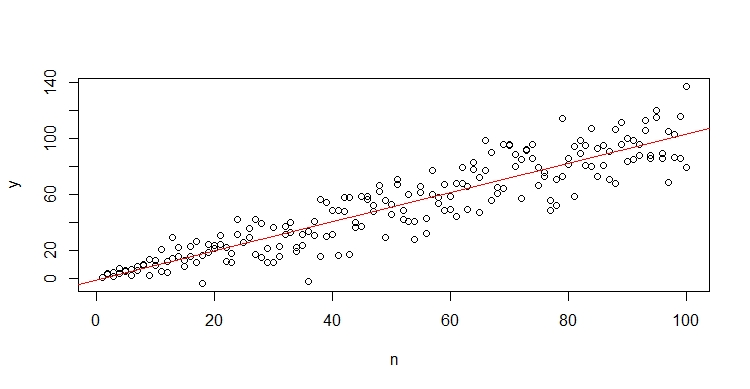
\includegraphics[scale=.6]{images/heteroscedasticity-own-ref}
\caption{Die Daten weisen im Zeitverlauf unterschiedliche Abweichung zur Trendgerade auf, d.h. die Residuen/Störterme sind nicht konstant im Zeitverlauf und es liegt Heteroskedastizität vor (Eigene Darstellung).}
\label{fig:heteroscedasticity}
\end{center}
\end{figure}

Eine Verallgemeinerung der ARCH-Modelle wurde 1986 von Tim Bollerslev in Form des GARCH($i$,$j$)-Modells beschrieben. Hier hängt die bedingte Varianz der zufälligen Modellfehler im Zeitpunkt $t$ nicht nur von Zufallsfehler der letzten $i$ Vorperioden ab, sondern auch von sich selbst, also der bedingten Varianz der $j$ vorherigen Zeitpunkte \parencite{bollerslev:1986}.\\
Sei $d_t$ eine Zeitreihe und $\epsilon_t$ das Residuum im Zeitpunkt $t$, dann gilt
\begin{align}
d_t&= \sigma_t\cdot \epsilon_t \nonumber \\
\sigma_t^2 &= a_0 + a_1d_{t-1}^2 + ... + a_id_{t-p}^2+b_1\sigma_{t-1}^2+ ... +b_j\sigma_{t-j}^2
\end{align} 
Wobei $a_l$, $b_k \in \mathbb{R}_{>0}$ mit  $a_i \neq 0$ und $b_j\neq 0$ gilt. Außerdem sind die Fehlerterme unabhängige identisch verteilte Zufallsvariablen mit $E(\epsilon_t)=0$ und $VAR(\epsilon_t)=1$. 
Somit gilt, dass die bedingte Varianz 
\[\sigma_t^2 = VAR(d_t|d_{t-1},d_{t-2},...)\]
sowohl von Werten der eigenen Vergangenheit als auch von der Vergangenheit der gesamten Zeitreihe abhängt.

In der Ökonometrie werden autoregressive Modelle z.B. für die Modellierung und Prognose von Finanzmarktdaten genutzt. Kurse an Finanzmärkten unterliegen in der Regel keiner gleichmäßigen Volatilität. Phasen mit geringen Schwankungen alternieren mit Phasen starker Schwankungen. Die Zeitreihenanalyse und insbesondere GARCH-Modelle dienen der Identifikation und Beschreibung dieser Volatilitätscluster. 

In dieser Arbeit wurde das GARCH(1,1)-Modell als Vergleichsmodell und Baseline berücksichtigt, da es ein in der Ökonometrie weitverbreitetes und genutztes Modell ist.

Beim GARCH(1,1)-Modell hängt die bedingte Varianz nur vom vorherigen Zeitpunkt ab und somit gilt 
\[\sigma_t^2 = VAR(d_t|d_{t-1})\]
Entsprechend kann die GARCH(1,1) Zeitreihe wie folgt modelliert werden:
\begin{align}
d_t &= \sigma_t\cdot \epsilon_t \nonumber \\
\sigma_t^2 &= a_0 + a_1d_{t-1}^2 + b_1\sigma_{t-1}^2
\end{align} 
Bei den untersuchten Zeitreihen in dieser Arbeit handelt es sich um Kursdaten des S\&P 500 Indexes (vgl. Kapitel~\ref{chap:data}), d.h. das GARCH(1,1)-Modell untersucht Volatilitätscluster dieser Preise. Die Preise wurden in Erträge $r_t$ umgerechnet, wobei je nach Markierung der Beobachtung der beobachtete Ertrag oder der geschätzte Ertrag $r_t$ verwendet wird.
\[r_t = \mu +\sigma_t\cdot \epsilon_t\]
Entsprechend kann das GARCH(1,1)-Modell zur Modellierung der Volatilität in Form der Standardabweichung der Erträge implementiert werden.

\begin{align}
\sigma_t^2 &= a_0 + a_1d_{t-1}^2 + b_1\sigma_{t-1}^2 \nonumber \\
\sigma_t^2 &=a_0+a_1(\sigma_t\cdot \epsilon_t)^2 + b_1\sigma_{t-1}^2\nonumber \\
\sigma_t^2 &=a_1(\sigma_{t-1}\cdot \epsilon_{t-1} +\mu -\mu)^2 +b_1\sigma_{t-1}^2 \nonumber \\
\sigma_t^2 &= a_0+a_1(r_{t-1}-\mu)^2 +b_1\sigma_{t-1}^2
\end{align} 
Die Berechnung wird entsprechend im \textit{Stan}-Code als  transformierter Parameter implementiert.
\begin{lstlisting}[style=custom]

parameters {
  real mu;
  real<lower=0> alpha0;
  real<lower=0,upper=1> alpha1;
  real<lower=0,upper=(1-alpha1)> beta1;
  real<lower=0> sigma1;
  real eps_miss[N]; // missing normalized return innovations
}
transformed parameters {
  real ret[T]; // returns ... observed or r_t = mu + sigma_t * eps_t
  real<lower=0> sigma[T];

  {
    int idx = 1; // missing value index

    sigma[1] = sigma1;
    if (miss_mask[1] == 1) {
      ret[1] = mu + sigma[1] * eps_miss[idx];
      idx = idx + 1;
    } else
      ret[1] = ret_obs[1];

    for (t in 2:T) {
      sigma[t] = sqrt(alpha0
                    + alpha1 * pow(ret[t - 1] - mu, 2)
                    + beta1 * pow(sigma[t - 1], 2));
      if (miss_mask[t] == 1) {
        ret[t] = mu + sigma[t] * eps_miss[idx];
        idx = idx + 1;
      } else
        ret[t] = ret_obs[t];
    }
  }
}

\end{lstlisting}
Der Erwartungswert $\mu$ sowie die Standardabweichung $\sigma$ sind standardnormalverteilt. Die Erträge folgen einer Normalverteilung mit den Parametern $\mu$ und $\sigma$. Außerdem muss die Ziel-Dichte die Jacobi-Korrektur (\textit{engl. Jacobian Correction}) für alle Vorhersagen berücksichtigen.
Schließlich wird im \verb|model|-block des \textit{Stan}-Codes, die a-posteriori-Dichte als normalisierte bedingte Verteilung der Erträge \verb|ret_obs| von $\mu$ und $\sigma$ definiert.

\begin{lstlisting}[style=custom]
model {
  mu ~ normal(0, 1);
  sigma1 ~ normal(0, 1);

  ret ~ normal(mu, sigma);
  // Jacobian correction for transformed innovations
  for (t in 1:T) {
    if (miss_mask[t] == 1)
      target += log(sigma[t]);
  }
}
generated quantities {
  real log_lik[T];

  for (t in 1:T)
    log_lik[t] = normal_lpdf(ret_obs[t] | mu, sigma[t]);
}
\end{lstlisting}
 
Der vollständige \textit{Stan}-Code des GARCH(1,1)-Modells befindet sich im Anhang~\ref{stan:GARCH}.

\section{Franke \& Westerhoff (FW)}
\label{chap:FW}
R. Franke und F. Westerhoff haben ein Modell entwickelt, dass den Markt durch zwei Agentengruppen bzw. Handelsstrategien beschreibt: Fundamental\footnote{\textbf{Fundamental-Trader} treffen Kauf bzw. Verkaufsentscheidung auf Basis vorhandener betriebswirtschaftlicher- und Kapitalmarktinformationen wie z.B. Jahresabschlüsse, Inflation, politische Informationen etc.. Für Fundamental-Trader gilt die Annahme, dass Märkte vorhersagbar sind und auf bestimmte Vorfälle vorhersagbares Verhalten zeigen. Durch Informationen über eben diese Vorfälle, kann der Händler informierte Vorhersagen über die Preise am Finanzmarkt treffen.}- und Chartist\footnote{\textbf{Chartist-Trader} treffen Handelsentscheidungen auf Basis historischer Preise und Volumen des Marktes. Chartist-Trader analysieren graphische Repräsentationen der historischen Daten und mathematische Indikatoren, um ihre Handelsstrategie zu optimieren.}-Trader. Händler können täglich die Strategie ändern, da im Modell ein Mechanismus modelliert wurde, der Herdenverhalten abbildet \parencite{FW:2011}\\
Der Anteil der Fundamental-Trader zum Zeitpunkt $t$ sei \[
n_t^f\in [0,1] \]
Dann gilt für den Anteil der Chartist-Trader entsprechend
\[n_t^c = 1-n_t^f\]
da nur zwei Handelsstrategien am Markt existieren\parencite{bertschinger:2018,FW:2011}.

Der logarithmierte Preis $p_t$ im Zeitpunkt $t$ hängt vom vorherigen Preis sowie der vorherigen durchschnittlichen Nachfrage aller Händler $d_{t-1}^f$ und $d_{t-1}^c$ ab. 
\begin{align}
p_t = p_{t-1} + \mu (n_{t-1}^f\cdot d_{t-1}^f + n_{t-1}^c\cdot d_{t-1}^c)
\end{align}
Fundamental-Trader reagieren auf fehlerhafte Preise z.B. wenn der Marktpreis vom (bekannten) Fundamentalpreis\footnote{Der \textbf{Fundamentalpreis} ist der Preis, der rein auf Basis vorhandener Informationen berechnet wurde} $p^*$ des Vermögenswertes abweicht. Chartist-Trader reagieren im Gegensatz dazu auf Preisbewegungen der Vergangenheit z.B. $p_t-p_{t-1}$.
Die Nachfrage selbst ist keine beobachtbare Größe und nur ihre gewichtete Summe beeinflusst die Preise. Sie wird von \parencite{bertschinger:2018,FW:2011} mittels folgender Dynamiken definiert:
\begin{align}
d_t^f &= \phi (p^*-p_t)+\epsilon_t^f & &\text{mit }\epsilon_t^f\sim \mathcal{N}(0,\sigma^2_f)\nonumber \\
d_t^c &= \xi (p_t-p_{t-1})+\epsilon_t^c & &\text{mit }\epsilon_t^c\sim \mathcal{N}(0,\sigma^2_c)\nonumber 
\end{align}
Allgemein gilt für zwei unabhängige Zufallsvariablen $X$, $Y$, dass die Verteilung ihrer Summe der Faltung der Verteilung der beiden Zufallsvariablen entspricht.\\
Sei
\begin{align}
X&\sim \mathcal{N}(\mu_X, \sigma_X^2)\nonumber \\
Y&\sim \mathcal{N}(\mu_Y,\sigma_Y^2)\nonumber
\end{align}
dann gilt
\[X+Y\sim\mathcal{N}(\mu_X+\mu_Y,\sigma_X^2+\sigma_Y^2)\]
So ist es möglich, dass die Nachfrage nicht tatsächlich berechnet bzw. geschätzt werden muss, sondern indirekt durch die Verteilung der kombinierte Nachfrage der existierenden Trader-Gruppen Einfluss auf die logarithmierten Preise $r_t = p_t-p_{t-1}$ nimmt.
Für das stochastische Modell der logarithmierten Preise 
\[r_t\sim\mathcal{N}(\mu_t,\sigma_t^2)\]
gelten dann die Verteilungsparamter
\begin{align}
\mu_t&= E[n_{t-1}^f\; d_{t-1}^f + n_{t-1}^c\; d_{t-1}^c]\nonumber\\
&=\mu (n_{t-1}^f\; \phi(p^*-p_{t-1}) +n_{t-1}^c\; \xi (p_{t-1}+p_{t-2}))
\end{align}
und
\begin{align}
\label{eq:FW-vol}
\sigma_t^2 &= \mu^2((n_{t-1}^f)^2\sigma_f^2 + (n_{t-1}^c)^2\sigma_c^2)
\end{align}
Die Volatilität $\sigma_t$ hängt somit von der Größe der einzelnen Trader-Gruppen ab und ändert sich mit der Zeitreihe. Um den Wechsel der Händler von einer Gruppe zur Anderen zu beschreiben, wird zu jedem Zeitpunkt $t$ deren Anteil am Gesamtmarkt  $n_t^f$ bzw. $n_t^c$ neu berechnet.
Der Aktualisierungs-Quotient in Formel~\ref{eq:FW-update} entspricht der DCA\footnote{\textbf{Discrete Choice Approach}(DCA) nach Formel~\ref{eq:FW-update} \parencite{bertschinger:2018}}-HPM\footnote{\textbf{Herding, Predisposition, Missalignment}(HPM) Spezifikation für Attraktivität der Fundamental-Strategie gegenüber der Chartist-Strategie\parencite{bertschinger:2018}.} Spezifikation nach \parencite{bertschinger:2018, FW:2011}.\\

Sei $a_t$ die relative Attraktivität der Fundamental-Strategie gegenüber der Chartist-Strategie. Nach \parencite{bertschinger:2018, FW:2011} wird die Attraktivtät mittels drei beeinflussender Faktoren modelliert (vgl. Formel~\ref{eq:FW-att}). 
Zum einen wird eine allgemeine Veranlagung (General Predisposition) $\alpha_0$ und zum anderen Herdenverhalten (Herding) $\alpha_n$ und fehlerhafte Preise $\alpha_p$ modelliert (HPM).
Da nur eine diskrete Anzahl an Wahlmöglichkeiten bestehen (DCA), ist die Wahrscheinlichkeitsdichte des Modells leicht differenzierbar. Das hat zur Folge, dass ein HMC-Algorithmus leichter Stichproben aus der a-posterior-Verteilung ziehen kann.\\
Wie bereits erwähnt gilt \[n_t^c = 1-n_t^f\]
wobei die Veränderung der Anzahl der Händler zu jedem Zeitpunkt $t$ durch den inversen Logit\footnote{Der \textbf{Logit} entspricht dem natürlichen Logarithmus der Wahrscheinlichkeit einer Chance (Quotient der Wahrscheinlichkeit $p$ zur Gegenwahrscheinlichkeit $1-p$). Für die Inverse gilt $p=\frac{e^X}{1+e^X}=\frac{1}{1+e^{-X}}$ \parencite{logit}} berechnet wird (vgl. Code~\ref{stan:FW-param} Zeile~\ref{stan:FW-param:logit})
\begin{align}
\label{eq:FW-update}
n_t^f =\dfrac{1}{1+e^{-\beta\cdot a_{t-1}}} && \beta = 1\text{ nach \parencite{bertschinger:2018}}
\end{align}
mit
\begin{align}
\label{eq:FW-att}
a_t= \alpha_0+\alpha_n(n_t^f-n_t^c)+\alpha_p(p^*-p_t)^2 &&a_n, a_p >0
\end{align}
Im \textit{Stan}-Code werden die Paramter entsprechend im \verb|parameter|- bzw. \verb|transformed parameter|-Block definiert.
\begin{lstlisting}[style=custom, escapechar=|,caption={Teil-Modell nach \parencite{bertschinger:2018, FW:2011}},label={stan:FW-param}]
parameters {
  real<lower=0> phi;
  real<lower=0> xi;
  real alpha_0;
  real<lower=0> alpha_n;
  real<lower=0> alpha_p;
  real<lower=0> sigma_f;
  real<lower=sigma_f> sigma_c;
  real<lower=0, upper=1> n_f_1;
  ...
  vector[N] eps_miss; // missing normalized return innovations
}
transformed parameters {
  vector[T] n_f;
  vector[T] demand;
  vector[T] sigma;
  // Note: All prices are actually log prices!
  vector[T] p_star;
  vector[T] p;
  real ret[T];
  ...
  
  p[1] = 0; // wlog log p_1 = 0
  p_star[1] = ...
  
  n_f[1] = n_f_1;
  demand[1] = 0;
  
  sigma[1] = mu * sqrt( square(n_f[1] * sigma_f)
			+ square((1 - n_f[1]) * sigma_c));
  {
    int idx = 1;
    
    if (miss_mask[1] == 1) {
      ret[1] = sigma[1] * eps_miss[idx];
      idx = idx + 1;
    } else
      ret[1] = ret_obs[1];

    for (t in 2:T) {
      // Note: index shift between prices and returns
      p[t] = p[t - 1] + ret[t - 1];
      p_star[t] = ...

      {
	
    // equation (HPM)
	real a = alpha_n * (n_f[t-1] - (1 - n_f[t-1]))
	  + alpha_0
	  + alpha_p * square(p[t-1] - p_star[t-1]);
	
    // equation (DCA)
	n_f[t] = inv_logit(beta * a); |\label{stan:FW-param:logit}|
	
    demand[t] = mu * (n_f[t] * phi * (p_star[t] - p[t])
			  + (1 - n_f[t]) * xi * (p[t] - p[t-1]));
	
    // structured stochastic volatility
	sigma[t] = mu * sqrt( square(n_f[t] * sigma_f)
			      + square((1 - n_f[t]) * sigma_c));
      }
      
      if (miss_mask[t] == 1) {
        ret[t] = sigma[t] * eps_miss[idx];
        idx = idx + 1;
      } else
        ret[t] = ret_obs[t];
    }
  }
}
\end{lstlisting}

Die Parameter $\beta$ und $\mu$ sind redundante Parameter werden konstant gehalten, da sie nur die Größenordnung der Parameter $\alpha_0,\alpha_n,\alpha_p, f, g, \sigma_f$ und $\sigma_c$ beeinflussen. \\
Es gilt
\[\beta = 1\]
\[\mu = 0.01\]
Die Definition der Parameter wird im \textit{Stan}-Code im \verb|transformed data|-Block angelegt. Also enthält dieser neben der Berechnungsvorschrift der \textit{Missing Values} auch die Vorschrift für $\sigma_t$, $\mu$ und $\beta$.
\begin{lstlisting}[style=custom]
transformed data {
  int N = 0; // number of missing values
  real ret_sd  = sqrt(variance(ret_obs));
  // mu and beta fixed ... redundant anyways
  real mu = 0.01;
  real beta = 1.0;

  for (t in 1:T)
    if (miss_mask[t] == 1) N = N + 1;
}
\end{lstlisting}
Das Model wird anschließend im \verb|model| bzw. \verb|generated quantities|-Block mit finalisiert. Da wenig Wissen über die korrekte Wahl der a-priori-Verteilung für alle Parameter vorliegt, werden diese mit wenig informativen Verteilungen initialisiert, die die Skala der Parameter bestimmt. Dazu wurde die Studentsche t-Verteilung (vgl. Abbildung~\ref{fig:student-t}) gewählt, da diese schwere Ränder hat. So werden Werte, die um ein Vielfaches größer als die Standardabweichung sind, dennoch akzeptiert. Lediglich die Standardabweichungen folgen stärker informierte a-prori-Verteilungen auf Basis der Daten. Wie bereits in Kapitel~\ref{chap:garch} beschrieben wird auch hier die Jacobi-Korrektur modelliert. 
%img student-t
\begin{figure}[H]
\begin{center}
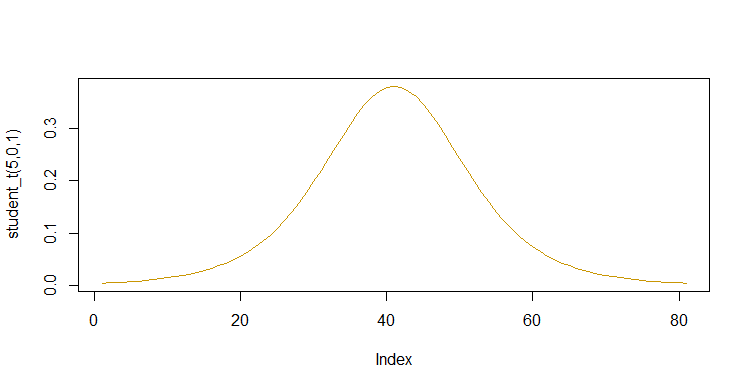
\includegraphics[scale=.5]{images/student_t}
\caption{Die Studentsche t-Verteilung mit 5 Freiheitsgraden, dem Erwartungswert 0 skaliert um den Faktor 1 (Eigene Darstellung).}
\label{fig:student-t}
\end{center}
\end{figure}

\begin{lstlisting}[style=custom]
model {
  phi ~ student_t(5, 0, 1);
  xi ~ student_t(5, 0, 1);
  alpha_0 ~ student_t(5, 0, 1);
  alpha_n ~ student_t(5, 0, 1);
  alpha_p ~ student_t(5, 0, 1);
  sigma_f ~ normal(0, ret_sd / mu);
  sigma_c ~ normal(0, 2.0 * ret_sd / mu);
  ...

  // Price likelihood
  ret ~ normal(demand, sigma);
  // Jacobian correction for transformed innovations
  for (t in 1:T) {
    if (miss_mask[t] == 1)
      target += log(sigma[t]);
  }
}
generated quantities {
  vector[T] log_lik;

  for (t in 1:T)
    log_lik[t] = normal_lpdf(ret_obs[t] | 0, sigma[t]);
}
\end{lstlisting}

Außerdem wird angenommen, dass der Fundamentalpreis unbekannt und nicht beobachtbar ist, das wird durch den logarithmierte Fundamentalpreis $p^*=0$ modelliert \parencite{bertschinger:2018, FW:2011}. Bei der Simulation des Modells auf realen Aktienmarktpreisen bzw. -erträgen, wird angenommen, dass sich der Fundamentalpreis im Zeitverlauf ändert.

Des Weiteren gilt, dass die Volatilität $\sigma_t$ in Formel~\ref{eq:FW-vol} über den Marktanteil der Fundamental-Trader $n_{t-1}^f$ von der Attraktivität $a_{t-2}$ in Formel~\ref{eq:FW-att} abhängt. Die Attraktivität wiederum wird vom logarithmierten Fundamentalpreis $p_{t-2}^*$ beeinflusst. \\ 

In der vorliegenden Arbeit wurden zwei verschiedene Varianten des Modells nach \parencite{bertschinger:2018} auf Marktpreisen simuliert. Die Varianten unterscheiden sich in der Berechnung der Änderungen des logarithmierten Fundamentalpreises $p_t^*$:
\begin{enumerate}
\item Modellierung von $p_t^*$ durch die Brownsche Bewegung bzw. eine Re-Parametrierung und die Berechnung mittels zufälliger Irrfahrt (Random Walk)
\item Modellierung von $p_t^*$ durch einen gleitenden Durchschnitt (Moving Average)
\end{enumerate}
In der ersten Variante wird angenommen, dass $p_t^*$ im Zeitverlauf der geometrischen Brownschen Bewegung\footnote{Die \textbf{Brownsche Bewegung} ermöglicht die Simulation multiplikativer unabhängiger Zuwächse des Fundamentalpreises \parencite{BrownianMotion}} folgt.
\begin{align}
\label{eq:FW-p_star}
p^*\sim \mathcal{N}(p_{t-1}^*,\sigma_*^2)
\end{align}

So enthält $p_t^*$ durch die Brownsche Bewegung nun eine stochastische Komponente. Da $p_t^*$ die Volatilität $\sigma_t$ beeinflusst, handelt sich also um ein stochastisches Volatilitätsmodell \parencite{bertschinger:2018, FW:2011}.\\ 

Durch eine nicht zentrierte Umparametrierung nach \parencite{bertschinger:2018} kann die Performance des HCM-Sampler verbessert werden. Dazu wird $p_t^*$ mittels $\epsilon_t^*$ als transformierter Parameter innerhalb einer zufälligen Irrfahrt (Random Walk) berechnet.
\begin{align}
\label{eq:FW-P_star-new}
p_t^* = p_{t-1}^*+\sigma_*\cdot\epsilon_t^* &&\text{ wobei }\epsilon_t^*\sim \mathcal{N}(0,1)
\end{align}
Das Modell bleibt dadurch unverändert, denn Formel~\ref{eq:FW-p_star} und~\ref{eq:FW-P_star-new} sind äquivalent \parencite{bertschinger:2018}.\\

Die erste Variante des Modells $\Theta_{FWwalk}$ wird also durch die Parameter $\epsilon_t^*$ und $\sigma_*$ ergänzt. Im \textit{Stan}-Code~\ref{stan:FWwalk-param} ist diese Variante entsprechend im \verb|parameter|- und \verb|transformed parameter|-Block in Zeile~\ref{stan:FWwalk-pstar} umgesetzt.

\begin{lstlisting}[style=custom, escapechar=|,caption={Teil-Modell(Random Walk) nach \parencite{bertschinger:2018, FW:2011}},label={stan:FWwalk-param}]
parameters {
  ...
  // p_star random walk in non-centered parameterization
  vector[T] epsilon_star;
  real<lower=0> sigma_p_star;
  ...
}
transformed parameters {
  ...
  vector[T] p_star;
  vector[T] p;
  ...

  p[1] = 0; 
  p_star[1] = p[1] + epsilon_star[1]; 

      ...

    for (t in 2:T) {
      // Note: index shift between prices and returns
      p[t] = p[t - 1] + ret[t - 1];
      p_star[t] = p_star[t-1] + sigma_p_star * epsilon_star[t]; |\label{stan:FWwalk-pstar}|     

      {
	...
  }
\end{lstlisting}

Der vollständige \textit{Stan}-Code der ersten Variante befindet sich im Anhang~\ref{stan:FWwalk}.\\

In Variante 2 wird die Veränderung des logarithmierten Fundamentalpreises durch einen gleitenden Durchschnitt modelliert. Es wird angenommen, dass der Fundamentalpreis von aktuellen sowie vergangenen Werten eines unbekannten stochastischen Terms (Zufallsfehler) abhängt. Auch für diese Variante gilt somit, dass es sich um ein stochastisches Volatilitätsmodell handelt \parencite{bertschinger:2018}. Der vollständige \text{Stan}-Code befindet sich im Anhang~\ref{stan:FWma}.\\

random walk - treedepth 128 ?!

\section{AL herd walk (AL)}
\label{chap:AL}
tbd

\chapter{Simulationen}
\label{chap:sim}
tbd

\section{Daten \& Vorhersagen}
\label{chap:data}
S\&P 500 data in USD from finance.yahhoo: \\ 
-daily prices - calculated into return and finally into log return as models expect log return as inputs\\
-exporting data with dates like Jan 1 2000 to Jan 1 2008 yahoo automatically uses last working day at stock exchange\\
- always used 30 Predictions - inaccurate as days per month change\\
=> this all leads to inaccurancy which is ok as the goal is to see the tendency in which way predictions are shifting \\\\
monthly prediction during a year in which a major crisis happend: bank crisis 2008 \& dotcom 2000?\\
used 8 years to predict the year 2008 on a monthly basis: e.g. data from Jan 1 2000 to Jan 1 2008 used to predict Jan 2008

\section{Ergebnisse}
\label{chap:results}
tbd

\includegraphics[scale=.6]{../plots/bank-crisis/AL_walk/01_AL_walk_Jan_low_info_depth-13_delta_9}

%\printbibliography
%\listoffigures

\appendix

\chapter*{Anhang}
\addcontentsline{toc}{chapter}{Anhang}

\addtocontents{toc}{\protect\setcounter{tocdepth}{1}} %don't display subsections in toc

\renewcommand{\thesection}{\Alph{section}}

\section{\textit{Stan} Code}
\subsection{GARCH-Modell}
\label{stan:GARCH}
\begin{lstlisting}[style=custom]
data {
  int<lower=0> T;
  int<lower=0, upper=1> miss_mask[T];
  real ret_obs[T]; // Note: Masked indices will be treated as missing;
}
transformed data {
  int N = 0; // number of missing values
  for (t in 1:T)
    if (miss_mask[t] == 1) N = N + 1;
}
parameters {
  real mu;
  real<lower=0> alpha0;
  real<lower=0,upper=1> alpha1;
  real<lower=0,upper=(1-alpha1)> beta1;
  real<lower=0> sigma1;
  real eps_miss[N]; // missing normalized return innovations
}
transformed parameters {
  real ret[T]; // returns ... observed or r_t = mu + sigma_t * eps_t
  real<lower=0> sigma[T];

  {
    int idx = 1; // missing value index

    sigma[1] = sigma1;
    if (miss_mask[1] == 1) {
      ret[1] = mu + sigma[1] * eps_miss[idx];
      idx = idx + 1;
    } else
      ret[1] = ret_obs[1];

    for (t in 2:T) {
      sigma[t] = sqrt(alpha0
                    + alpha1 * pow(ret[t - 1] - mu, 2)
                    + beta1 * pow(sigma[t - 1], 2));
      if (miss_mask[t] == 1) {
        ret[t] = mu + sigma[t] * eps_miss[idx];
        idx = idx + 1;
      } else
        ret[t] = ret_obs[t];
    }
  }
}
model {
  mu ~ normal(0, 1);
  sigma1 ~ normal(0, 1);

  ret ~ normal(mu, sigma);
  // Jacobian correction for transformed innovations
  for (t in 1:T) {
    if (miss_mask[t] == 1)
      target += log(sigma[t]);
  }
}
generated quantities {
  real log_lik[T];

  for (t in 1:T)
    log_lik[t] = normal_lpd\phi (ret_obs[t] | mu, sigma[t]);
}


\end{lstlisting}
\subsection{Modell von Franke \& Westerhoff (Random Walk)}
\label{stan:FWwalk}
\begin{lstlisting}[style=custom]
data {
  int<lower=0> T; // time points (equally spaced)
  int<lower=0, upper=1> miss_mask[T];
  vector[T] ret_obs; // Note: Masked indices will be treated as missing;
}
transformed data {
  int N = 0; // number of missing values
  real ret_sd  = sqrt(variance(ret_obs));
  // mu and beta fixed ... redundant anyways
  real mu = 0.01;
  real beta = 1.0;

  for (t in 1:T)
    if (miss_mask[t] == 1) N = N + 1;
}
parameters {
  real<lower=0> phi;
  real<lower=0> xi;
  real alpha_0;
  real<lower=0> alpha_n;
  real<lower=0> alpha_p;
  real<lower=0> sigma_f;
  real<lower=sigma_f> sigma_c;
  real<lower=0, upper=1> n_f_1;
  // p_star random walk in non-centered parameterization
  vector[T] epsilon_star;
  real<lower=0> sigma_p_star;
  vector[N] eps_miss; // missing normalized return innovations
}
transformed parameters {
  vector[T] n_f;
  vector[T] demand;
  vector[T] sigma;
  // Note: All prices are actually log prices!
  vector[T] p_star;
  vector[T] p;
  real ret[T];

  p[1] = 0; // wlog log p_1 = 0
  p_star[1] = p[1] + epsilon_star[1]; // fixme ... interpretation epsilon_raw[1]
  
  n_f[1] = n_f_1;
  demand[1] = 0;
  sigma[1] = mu * sqrt( square(n_f[1] * sigma_f)
			+ square((1 - n_f[1]) * sigma_c));
  {
    int idx = 1;
    
    if (miss_mask[1] == 1) {
      ret[1] = sigma[1] * eps_miss[idx];
      idx = idx + 1;
    } else
      ret[1] = ret_obs[1];

    for (t in 2:T) {
      // Note: index shift between prices and returns
      p[t] = p[t - 1] + ret[t - 1];
      p_star[t] = p_star[t-1] + sigma_p_star * epsilon_star[t];      

      {
	// equation (HPM)
	real a = alpha_n * (n_f[t-1] - (1 - n_f[t-1]))
	  + alpha_0
	  + alpha_p * square(p[t-1] - p_star[t-1]);
	// equation (DCA)
	n_f[t] = inv_logit(beta * a);
	demand[t] = mu * (n_f[t] * phi * (p_star[t] - p[t])
			  + (1 - n_f[t]) * xi * (p[t] - p[t-1]));
	// structured stochastic volatility
	sigma[t] = mu * sqrt( square(n_f[t] * sigma_f)
			      + square((1 - n_f[t]) * sigma_c));
      }
      
      if (miss_mask[t] == 1) {
        ret[t] = sigma[t] * eps_miss[idx];
        idx = idx + 1;
      } else
        ret[t] = ret_obs[t];
    }
  }
}
model {
  phi ~ student_t(5, 0, 1);
  xi ~ student_t(5, 0, 1);
  alpha_0 ~ student_t(5, 0, 1);
  alpha_n ~ student_t(5, 0, 1);
  alpha_p ~ student_t(5, 0, 1);
  sigma_f ~ normal(0, ret_sd / mu);
  sigma_c ~ normal(0, 2.0 * ret_sd / mu);
  epsilon_star ~ normal(0, 1);
  sigma_p_star ~ normal(0, ret_sd / 2.0);
  
  // Price likelihood
  ret ~ normal(demand, sigma);
  // Jacobian correction for transformed innovations
  for (t in 1:T) {
    if (miss_mask[t] == 1)
      target += log(sigma[t]);
  }
}
generated quantities {
  vector[T] log_lik;

  for (t in 1:T)
    log_lik[t] = normal_lpd\phi (ret_obs[t] | 0, sigma[t]);
}

\end{lstlisting}

\subsection{Modell von Franke \& Westerhoff (Moving Average)}
\label{stan:FWma}
\begin{lstlisting}[style=custom]
data {
  int<lower=0> T; // time points (equally spaced)
  int<lower=0, upper=1> miss_mask[T];
  vector[T] ret_obs; // Note: Masked indices will be treated as missing;
}
transformed data {
  int N = 0; // number of missing values
  real ret_sd  = sqrt(variance(ret_obs));
  // mu and beta fixed ... redundant anyways
  real mu = 0.01;
  real beta = 1.0;

  for (t in 1:T)
    if (miss_mask[t] == 1) N = N + 1;
}
parameters {
  real<lower=0> phi;
  real<lower=0> xi;
  real alpha_0;
  real<lower=0> alpha_n;
  real<lower=0> alpha_p;
  real<lower=0> sigma_f;
  real<lower=0> sigma_c;
  real<lower=0, upper=1> n_f_1;
  real<lower=0> lenscale_raw;  
  real p_star_0;
  vector[N] eps_miss; // missing normalized return innovations
}
transformed parameters {
  vector[T] n_f;
  vector[T] demand;
  vector[T] sigma;
  // Note: All prices are actually log prices!
  vector[T] p_star;
  vector[T] p;
  real ret[T];
  real<lower=0> lenscale = 1000 * lenscale_raw;
  real<lower=0, upper=1> tau = exp( - 1 / lenscale);

  p[1] = 0; // wlog log p_1 = 0
  p_star[1] = log_mix(tau, p_star_0, p[1]);
  
  n_f[1] = n_f_1;
  demand[1] = 0;
  sigma[1] = mu * sqrt( square(n_f[1] * sigma_f)
			+ square((1 - n_f[1]) * sigma_c));
  {
    int idx = 1;
    
    if (miss_mask[1] == 1) {
      ret[1] = sigma[1] * eps_miss[idx];
      idx = idx + 1;
    } else
      ret[1] = ret_obs[1];

    for (t in 2:T) {
      // Note: index shift between prices and returns
      p[t] = p[t - 1] + ret[t - 1];
      p_star[t] = log_mix(tau, p_star[t-1], p[t]);

      {
	// equation (HPM)
	real a = alpha_n * (n_f[t-1] - (1 - n_f[t-1]))
	  + alpha_0
	  + alpha_p * square(p[t-1] - p_star[t-1]);
	// equation (DCA)
	n_f[t] = inv_logit(beta * a);
	demand[t] = mu * (n_f[t] * phi * (p_star[t] - p[t])
			  + (1 - n_f[t]) * xi * (p[t] - p[t-1]));
	// structured stochastic volatility
	sigma[t] = mu * sqrt( square(n_f[t] * sigma_f)
			      + square((1 - n_f[t]) * sigma_c));
      }
      
      if (miss_mask[t] == 1) {
        ret[t] = sigma[t] * eps_miss[idx];
        idx = idx + 1;
      } else
        ret[t] = ret_obs[t];
    }
  }
}
model {
  phi ~ student_t(5, 0, 1);
  xi ~ student_t(5, 0, 1);
  alpha_0 ~ student_t(5, 0, 1);
  alpha_n ~ student_t(5, 0, 1);
  alpha_p ~ student_t(5, 0, 1);
  sigma_f ~ normal(0, ret_sd / mu);
  sigma_c ~ normal(0, 2.0 * ret_sd / mu);
  p_star_0 ~ normal(0, 0.2);
  lenscale_raw ~ inv_gamma(2, 1); // avoid lower boundary ... lenscale ~ inv_gamma(2, 1000)

  // Price likelihood
  ret ~ normal(demand, sigma);
  // Jacobian correction for transformed innovations
  for (t in 1:T) {
    if (miss_mask[t] == 1)
      target += log(sigma[t]);
  }
}
generated quantities {
  vector[T] log_lik;

  for (t in 1:T)
    log_lik[t] = normal_lpdf(ret_obs[t] | 0, sigma[t]);
}
\end{lstlisting}

\section{\textit{R} Code}
\begin{lstlisting}[style=custom]
data {
  int<lower=0> T;
  int<lower=0, upper=1> miss_mask[T];
  real ret_obs[T]; // Note: Masked indices treated as missing
}
transformed data {
  int N = 0; // number of missing values
  for (t in 1:T)
    if (miss_mask[t] == 1) N = N + 1;
}

\end{lstlisting}

\printbibliography

% predefined "Erklärung" from Prüfungsamt
\newpage

\chapter*{Eigenständigkeitserklärung}
%add to content table withouth number
\addcontentsline{toc}{chapter}{Eigenständigkeitserklärung}
\small{gemäß Bachelor-Ordnung Informatik 2011 §25 Abs. 11}\par\bigskip
\begin{minipage}{\linewidth}\large\par\vskip2cm
Hiermit erkläre ich Frau \par\vskip1cm
\rule{13cm}{0.6pt}\par
\vskip1cm
Die vorliegende Arbeit habe ich selbständig und ohne Benutzung anderer als der angegebenen Quellen und Hilfsmittel verfasst.\par\vskip3cm
Frankfurt am Main, den \rule{6cm}{0.6pt}\par
\vskip3cm
\rule{8cm}{0.6pt}\\
Unterschrift
\end{minipage}

\end{document}

